\newpage
\section{Motivation}
\label {sec:motiv}
In this section, we explain the developement process of a highly
available application in \tool. We discuss a simple case of anomilies
possible under
eventual consistency and then explain the difficulties associated 
with the ad-hoc anomaly prevention techniques.
Lastly we will explain how we generalized and automated such techniques
in our tool \tool, and liberated 
the developers from all the mentioned problems.
Our programming model will be completed in section
\ref{sec:ctrt_language}, where we introduce our specification  language,
that
allows developers fine tune \tool according to \emph{any} 
anomaly witnessed in EC stores.
%
%--- What is the application, what are the requirements 
%
\subsection{RDTs in Eventually Consistent Stores }
\begin{figure}[t]
        \centering
	\begin{subfigure}[b]{0.489\textwidth}
	\begin{lstlisting}
type Effect = String 
type State =  String 

read :: State -> (String,Maybe Effect)
read s = (s,Nothing)

write :: String -> ((),Maybe Effect)
write comment = ((),comment)

apply :: State -> Effect -> State 
apply s eff = in s ++ " - " ++ comment
	\end{lstlisting}
	\caption{A simple implementation}
	\label{subfig:comment_code}
	\end{subfigure}
	\hfill
	\begin{subfigure}[b]{0.475\textwidth}
	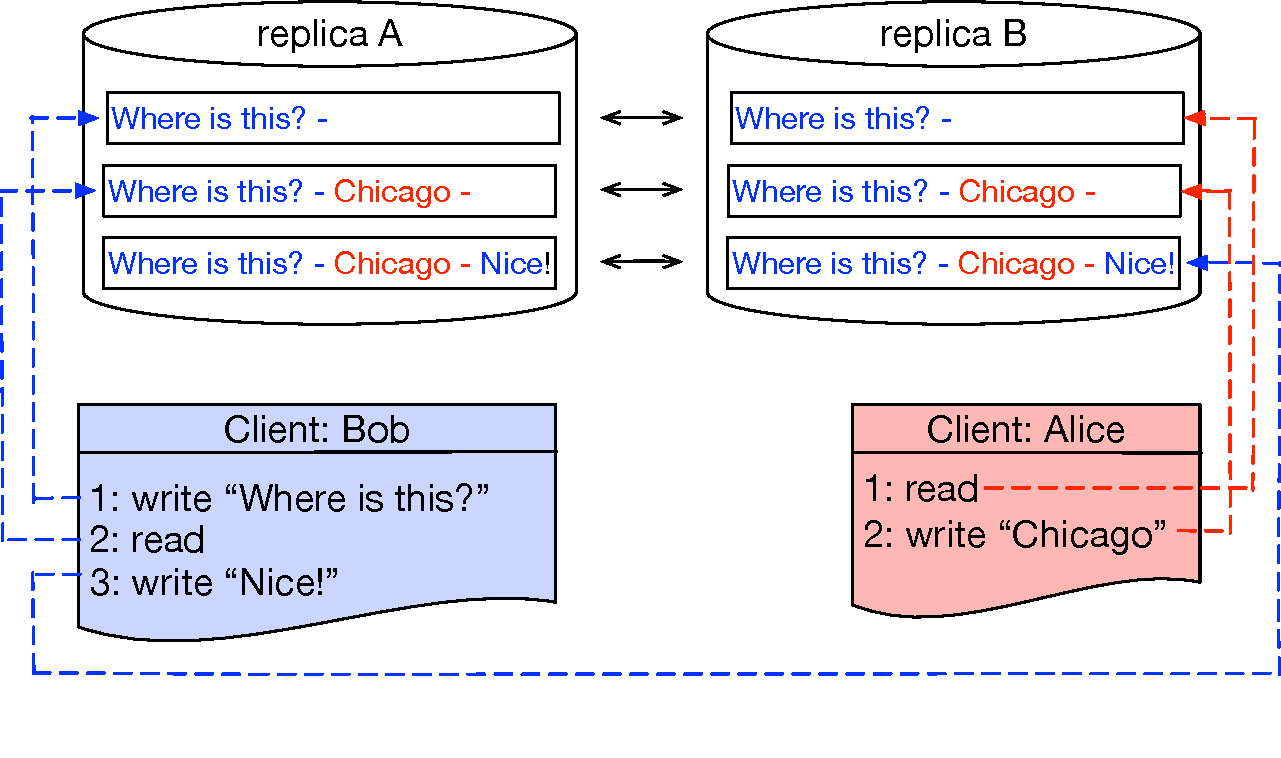
\includegraphics[scale=0.282]{Figures/comment_application.pdf}
	\caption{Example execution}
	\label{subfig:comment_example}
	\end{subfigure} 
\\ \hrulefill
\caption{A distributed application for comment section
management}
\label{fig:comment_app}
\end{figure}



Let's now consider a highly available application that manages the comment
section of posts, as part of a photo sharing web site.
Figure \ref{subfig:comment_code} presnets implementation of such an application
in our system model. As explained in section \ref{sec:sys_model}, the
code is consisted of types \effectC{} and \stateC{}. Both types here are
defined as strings, the former representing the text of a comment, and
the latter all the visible comments under a post, concatinated together.
A new \effectC{} is generated every time a user wants to comment on a
post by calling the \writeC{} function, and a \readC{} call simply
returns the \stateC{} of the object at the serving replica.

The \applyC{} function is given an effect, and is defined by the
developers to \emph{update} the objects' state.
Here the \applyC{} function simply pastes the 
included comment inside of  an effect, to the end of the current \stateC{}. As we mentioned earlier, we
completely separate the convergence semantics of the application  from the consistency
requirements. Since our focus is consistency here, we omit any conflict
resolution strategy in the code, however, developers (using roll-backs,
etc) can design the \applyC{} function to resolve conflicting
concurrent updates as they desire. 

Figure \ref{subfig:comment_example}, presents an example of how users
interact with the application. The example shows two clients, Bob and
Alice, that invoke operations on the same object. In the
beginning Bob writes a comment, which is routed to the replica A
(\ding{182}),
whose effect is then propagated and delivered to the replica B
(\ding{183}), where Alice's
first read operation is routed to next (\ding{184}). Alice and Bob then keep talking
through more read and write events while updates are being propagated between
replicas, whose order are marked in the
figure. 

Now let's assume Bob's read opration instead of replica A, was routed
to another replica C, where the update from his first operation was not
present. This is known as \emph{lost-updates} anomaly, a very
well-understood
undesired behavior that is admitted in eventually consistent stores. 
Now developers are faced with the problem of preventing such an undesired
behavior. A task that as we will explain shortly, is difficult,
erorneous and heavily tangled with the application logic.
%
%--- What are the challenges implementing those reuquirements manually
%
\subsection{Ad-hoc Anomaly Prevention}
In this part, by referring to the modified application  presented in figure
\ref{fig:modified_code}, we will
explain a well-understood approach toward eliminating the lost-updates anomaly in
the  comment manager application dicussed earlier. For simplicity, we
assume there are only two clients using the system, Bob and Alice.

%tagging effects
First modification required in this technique is tagging effects and
operations with
unique identifiers, consisting of their originating session (Alice/Bob),
and an integer showing their
sequence number in the session ($line:1,2,3$). Thais is used by replicas to
record the set of effects, that are alerady present locally.
By this simple adjustment, the undesired anomaly would
be completely avoided, if operations would never be routed to replicas,
that do not contain all the effects from prior operations on their
session (we call such effects the dependencies of
the operation). 

%blocking
Since operations do not have any control over which replica they are
routed to, the above property can be achieved, if operations that are
routed to a replica that does not contain their dependencies, postpone
their execution, until such effects become available at that replica.
This technique that is called {\bf blocking}, guarantees the state
witnessed by oerations, \emph{at least} contains updates of the desired set
of dependencies.

Another technique called {\bf filteration} is also used to further realize
the above idea, by basically separating the set of effects that have
arrived to the replica (available effects), and the set of effects that have
arrived and also been applied to the state (filtered effects).
By this separation, replicas can filter the set of available effects before
applying them, so that only effects are applied to the state, that all
effects in session order with them, have already been applied.
This way, in order to maintain the set of all effects applied to the state, 
replicas should only  record the highest sequence
numbers from each session, since it
is guaranteed that the smaller ones are also already applied ($line:4$). 

Figure \ref{fig:modified_code} represents the blocking technique in the modified \readC{}
operation, where the result is only returned if the sequence number of
the operation is larger than the previously seen sequence number from
that session precisely by 1 ($line:9,11$). Otherwise, the function is blocked by
calling itself recursively ($line:10,12$).
Furthermore, the
filteration technique is used in the modified \applyC{} funciton, that only
updates the state, if the sequence number of the given effect is
larger than the highest previously applied effect from that session,  precisly
by 1 ($line:16,19$).
\begin{figure}[t]
	\centering
	\begin{subfigure}[t]{0.5\textwidth}
	\begin{lstlisting}
data Sess = Bob | Alice
type ID = (Sess,Int) 
type Effect= (ID,String)
type State = (String,Int,Int)
	
read :: ID -> State -> String
read (sess,seq) (st,sq1,sq2) = 
	case sess (*@\textcolor{blue}{of}@*) 
		Bob ->   if (seq==sq1+1) (*@\textcolor{blue}{then}@*) st
		         else read (sess,seq)(st,sq1,sq2)
		Alice -> if (seq==sq2+1) (*@\textcolor{blue}{then}@*) st
		         else read (sess,seq)(st,sq1,sq2)
	\end{lstlisting}		  
	\end{subfigure}
	%
	\hfill
        %
	\begin{subfigure}[t]{0.42\textwidth}
	\begin{lstlisting}[firstnumber=13]
	apply :: State -> Effect -> State 
	apply (st,sq1,sq2) ((sess,seq),cm) = 
	  case sess (*@\textcolor{blue}{of}@*) 
	    Bob ->   if (sq1==seq-1)
	             (*@\textcolor{blue}{then}@*) (st++cm,sq1+1,sq2)
	             else (st,sq1,sq2)
	    Alice -> if (sq2==seq-1)
	             (*@\textcolor{blue}{then}@*) (st++cm,sq1,sq2+1)
	             else (st,sq1,sq2)
	\end{lstlisting}		  
        \end{subfigure}

	\hrulefill
	\caption{Guarded Application to Prevent Lost-updates Anomaly
	When Serving Bob and Alice}
	\label{fig:modified_code}
\end{figure}




The above approach obviously requires fundamentall changes in the code
and caused 90\% of
the application had to be  rewritten. Additionally, the modifications are
heavily tangled with the application logic which is a problem for
developement and reasoning of large productions.

The major drawback of this approach however, is the fact that it requires
constant alterations in the state of the application when the sessions
come and go, which happens very frequently.
The application is now required to make
sure that a new field is created locally \emph{and} globally when 
new sessions are connected. This requires constant alterations on the
tables in the data store, and making sure that the tables globally are
altered before allowing session to actually start. This requires direct
synchronization between replicas, which degrades the performance and
availability of the application. 

To make the matter worse, in addition to the above difficulties,
new anomalies are constantly found in systems, which requires
developers to come-up with new non-trivial solutions. For example, in the
above application, another type of anomaly can occur when a third user
Chris, uses the application and submits a read, which is routed to a
replica D, that only contains the last write from Bob. Then Chris sees a
window containing "Me too!", which is an undesirable behavior. Now
developers are left with two options. First, they can find 
another ad-hoc solution, which would further pollute the
application logic, making all the existing reasonings obsolete. Second,
they can move the whole developement to another store, that offers
stronger forms of consistency, such as causal consistency which would
prevent such anomalies. However, as we will show in section
\ref{sec:eval}, this would result in performance loss and potential
costumer loss for crtical applications.

%
%--- What is our alternative approach
%
\subsection{An Alternative}
\begin{wrapfigure}{i}{0.2\textwidth}
\centering
	\vspace{-10mm}
	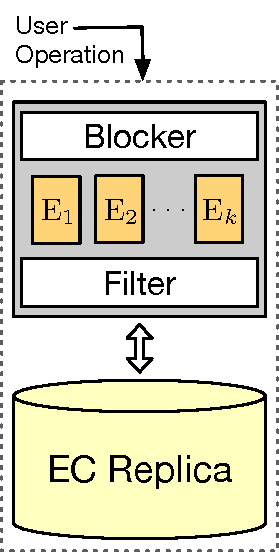
\includegraphics[scale=0.42]{Figures/outline.pdf}
	\label{fig:syncope_outline}
	\caption{\footnotesize \tool}
\label{fig:syncope_outline}
\vspace{-5mm}
\end{wrapfigure}



We now introduce our attractive alternative to the above ad-hoc solution. 
\tool, is our generic consistency managaement tool, running on
top of an off-the-shelf eventually consistent store, extending it to
a store with multiple configurable environments. 
Developers can define an environment for each operation at the
design stage, and configure each of them according to certain types of
anomalies, prevention of which in that environment is guaranteed by the
tool.
We have
relized this idea, following our observation that the prevention of basically all
types of anomalies, can be boiled down to two tasks,
filterataion and blocking. 

Our tool is equipped with a filteration mechanism, that periodically
refreshes the environments, and allows local effects at the replica to
enter each environment, if their presence would not result in the
occurence of the associated
anomaly. This way, \tool completely eliminates the
possibily of operations \emph{seeing effects that they are not supposed
to}, which is one important type of anomalies in distributed systems.
(for example, in the above example Chris was not supposed to see Bob's
last comment since some effects were missing from the replica).


Similarly, the tool contains a blocker mechanism that makes sure all
operations are executed on their associated environment only after the
environemnt includes the necessary effects for preventing the associated
anomaly. Consequently, the operations will \emph{always see the effects
that they are supposed to}. This eliminates another type of anomalies in
the distributed systems, that the lost-updates anomaly explained
previously, is an
example of. 


Using \tool, the developers are only required to configure environments
for each read operation, using a simple specification language that we
provide them with. The language is seeded with $\soZ$ $\visZ$ relations and allows
user to define different anomalous behaviors.  For example the
followings are the two consistency contracts written in our language,
regarding the two anomalies mentioned in this section:
\begin{smathpar}
\begin{array}{lllll}

\psi_1: & \forall (\eff,\eff'). & \eff \xrightarrow{\soZ} \eff' & \Rightarrow
& \eff
\xrightarrow {\visZ} \eff'  \\
\psi_2: & \forall(\eff,\eff'). & \eff \xrightarrow{\visZ;\visZ} \eff' &
\Rightarrow & \eff \xrightarrow {\visZ} \eff' 
\end{array}
\end{smathpar}


The first contract, that eliminates the possibility of lost\_updates,
tells the \tool to make sure that all effects that are in session order
to be also under visibility relation. This can be achieved by blocking
operations as explained above. 
The second contract, which prevents the second anomaly mentioned earlier,
requires the system to make sure that if an effect is being made visible
to an operation, the operation should also witness all effects that were
visible to that effect.
In the next section, we will formally introduce our specification
language, and explain how two types of anomalies mentioned above can be
transalated into contracts with different syntaxes.





















